\documentclass[a4paper,12pt,twoside,openright]{report}

\usepackage[utf8]{inputenc}
\usepackage[english]{babel}
\usepackage[T1]{fontenc}
\usepackage[backend=biber,sorting=none]{biblatex}
\usepackage[hidelinks]{hyperref}
\usepackage{amsmath}
\usepackage{blindtext}
\usepackage{color}
\usepackage{csquotes}
\usepackage{fancyhdr}
\usepackage{geometry}
\usepackage{graphicx}
\usepackage{lipsum}
\usepackage{listings}
\usepackage{pdfpages}
\usepackage{textcomp}
\usepackage{titlesec}

% ==== MARINGS, PARAGRAPHS, LINESPACE, TABLES, ETC. ====
\geometry{margin=3cm}
\setlength{\parskip}{0.7em}
\renewcommand{\baselinestretch}{1.5}

% ==== PAGE STYLING ====
\pagestyle{fancy}
\fancyhead{}
\fancyfoot[CE,CO]{}
\fancyfoot[LE,RO]{\thepage}

\definecolor{gray75}{gray}{0.75}
\newcommand{\PRLsep}{\noindent\makebox[\linewidth]{\resizebox{\linewidth}{1.5pt}{\textcolor{gray75}{$\bullet$}}}}
\renewcommand{\headrulewidth}{0pt}
\titleformat{\chapter}[hang]{\centering\Huge\bfseries}{\thechapter.\hspace{10pt}}{0pt}{\Huge\bfseries}[\vspace*{-0.7\baselineskip}\PRLsep]

% ==== BIBLIOGRAPHY ====
\addbibresource{bibliography.bib}

% ==== CODE SYNTAX HIGHLIGHTING ====

\definecolor{codegreen}{rgb}{0,0.6,0}
\definecolor{codemauve}{rgb}{0.58,0,0.82}
\lstset{
  upquote=true,
  numbers=left,
  backgroundcolor=\color{white},   
  basicstyle=\footnotesize,
  breaklines=true, 
  commentstyle=\color{codegreen},
  keywordstyle=\color{blue},
  stringstyle=\color{codemauve},
}

% ==== REAL DOCUMENT BEGINS HERE ====
\title{%
  \Huge FreyaFS \\
  \Large A virtual file system with Mix\&Slice support
}
\author{Michele Beretta}
\date{A.A. 2019/2020}

\begin{document}
  % ----- FRONTESPIZIO
  \thispagestyle{plain}  
  \pagenumbering{gobble}

  % ----- TITOLO
  \clearpage
  \maketitle
  
  % ----- EMPTY
  \clearpage
  \thispagestyle{plain}
  \pagenumbering{gobble}
  \mbox{}
  
  % ----- INDICE
  \clearpage
  \pagenumbering{Roman}
  \tableofcontents

  % ----- EMPTY
  \clearpage
  \thispagestyle{plain}
  \pagenumbering{gobble}
  \mbox{}

  \clearpage
  \pagenumbering{arabic}
  
  % ==================================================================
  % ====================== INTRODUZIONE ==============================
  % ==================================================================

  \chapter{Introduction}
  \thispagestyle{fancy}
  
  % Scrivere perché hai scelto la tesi e quale è stato il risultato (come ci sei arrivato)

  This thesis work describes the realisation of a virtual file system for GNU/Linux that supports
  the \textit{Mix\&Slice} encryption algorithm in a transparent way.

  This new file system will take care of creation, modification and deletion of files and folders.

  \section{Context}

  The main reason for the realisation of this encryption-supporting file system is data privacy.
  There are often files (or, more generally, information) that, because of confidentiality,
  we want to make accessible only to few selected people.
  This is simple to realise thanks to encryption, which allows to protect the desired information by making them
  available only to people who have a specific key.

  However, the usage and the access to this data should be as simple as possible, i.e.,
  it should be like accessing non-encrypted files.
  This functionality is realised by a virtual file system that encrypts and decrypts files
  on demand, hiding these operations from the user.

  \clearpage
  \section{The file system}

  \label{filesystem-descrizione}
  \subsection{Description}

  One of the most important functions of an operating system is taking care of information management on mass memory,
  which is any peripheral device other than central memory.
  The file system is the operating system module that implements this.
  In particular, the file system must \cite{sistemioperativi}:

  \begin{itemize}
    \item provide a unique and permanent identification mechanism for \textit{files},
          so that they can exist and be accessible for a long time;
    \item provide \textit{access methods} that allow addressing, reading and writing
          elementary blocks of information contained in the files;
    \item mask the physical characteristics of the storage units;
    \item implement access control mechanisms on files, both to ensure confidentiality of information and to avoid concurrency issues;
    \item guarantee the permanence and consistency of information even in the case of hardware or software malfunctions.
  \end{itemize}

  The main data structures a file system works with are file \textit{descriptors}.
  Descriptors contain various properties of the file, the main ones being its name and its address, i.e.,
  its position in mass memory.
  A set of descriptors is called \textit{directory} (or folder). Since directories also have to be
  stored on disk permanently, they are handled by Unix and Unix-like systems like files: more precisely,
  in the Unix system a directory is a file that contains the list of names and addresses of the files
  contained within.
  
  \clearpage
  \subsection{File operations}

  In order to access a file, its descriptor must be obtained from mass memory.
  However, this operation is computationally heavy in terms of the number of disk accesses.
  Hence, to solve this problem, the \textit{open} primitive is introduced: before any operation
  on the file, its descriptor is retrieved and its content transferred to main memory.
  This descriptor is then used to read and write the file in an efficient way.
  
  When no further operation needs to be performed, the inverse \textit{close} primitive is executed:
  the descriptor image contained in main memory is copied to disk, so to update the information
  contained in the file.

  We describe the opening of a file as the action of searching and copying in memory the descriptor of a file
  (and possibly its content), and the closing of a file as the release of the memory dedicated to
  the descriptor, resulting in the transfer of its content to disk.
  
  \subsection{Virtual file systems}

  A virtual file system is a software component that allows the operating system kernel to access the file system
  through the use of standard functions, independent from the actual file system (or the device used for storage).

  Access to file stored on other computers via the network, or access to encrypted files without the user
  noticing the encryption, are example where the virtual file system comes into play and simplifies the interaction
  between the user and the computer.

  \subsection{FUSE - File system in Userspace}

  FUSE is a software system that allows the creation of virtual file systems on the Linux kernel \cite{libfusegithub}.
  The FUSE project consists of two parts:
  \begin{enumerate}
    \item the kernel module for communicating with the Linux kernel;
    \item the \textit{libfuse} user library that implements the communication between the virtual file system and the kernel module.
  \end{enumerate}

  Therefore, FUSE allows the user to adopt directly the virtual file system mechanism on Linux and,
  in general, on Unix and Unix-like systems (including FreeBSD and macOS) thanks to a porting and rewriting process.

  \begin{figure}[h!]
    \centering
    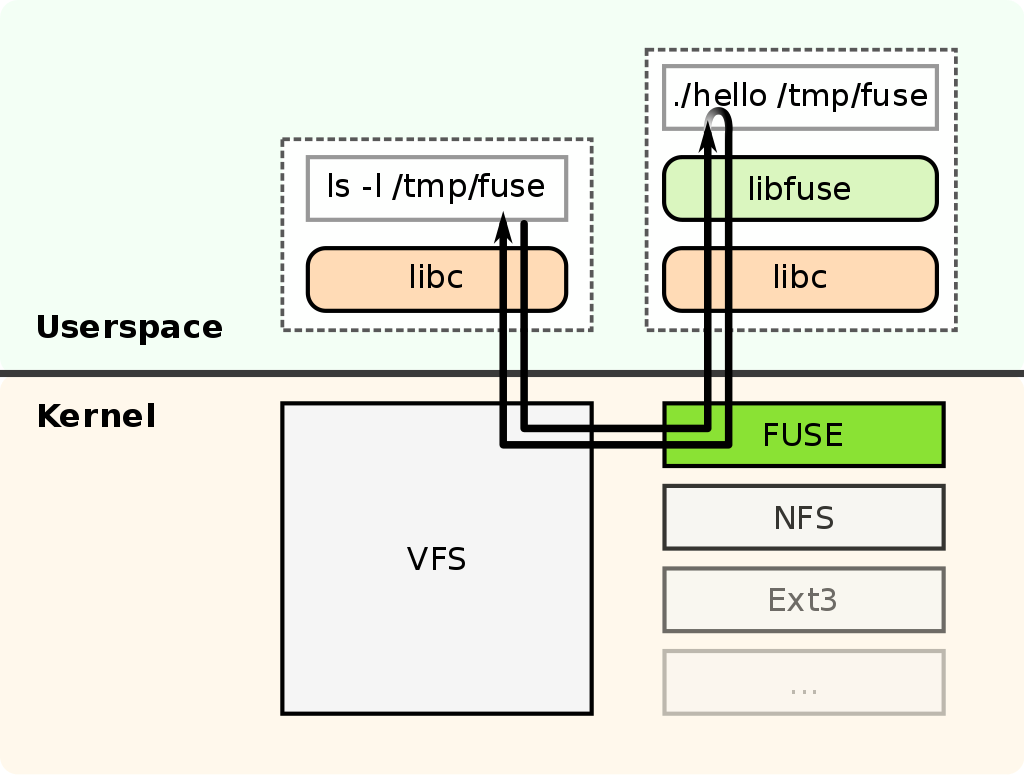
\includegraphics[width=0.6\linewidth]{images/fuse_structure.png}
    \caption{FUSE architecture}
    \label{fig:fuse-structure}
  \end{figure}

  Figure \ref{fig:fuse-structure} shows how FUSE interacts with the Linux kernel.
  
  Every request made from user space (\texttt{ls -l /tmp/fuse}) is intercepted by
  the VFS kernel module\footnotemark{} and is redirected to the FUSE kernel module.
  The request is then passed to the \textit{libfuse} userspace library, which runs a specific
  program configured to handle a request (\texttt{./hello}).
  The handler response is then sent back to FUSE, and finally forwarded to the initial program in userspace.

  \footnotetext{\textit{Virtual File System} \cite{linuxkernelvfs}, or \textit{Virtual File System Switch},
  a software layer of the Linux kernel that manages the interaction between userspace and the ``real'' file system.}

  \section{Cryptography}

  \subsection{Description and usage}

  \textit{Cryptography} is an algorithmic technique that allows to represent a message in a obscured way,
  in order to make it incomprehensible to anyone who is not permitted to read its content.
  The encrypted message is called \textit{cryptogram} and the used methods are called \textit{encryption techniques}.

  Cryptography is based on an algorithm and an encryption key. The algorithm is often public, while
  the encryption key is the information that guarantee the confidentiality of the message:
  without the key, it is not possible to access the encrypted information.

  This technique is used in many IT fields for various purposes, such as to guarantee privacy in a communication
  between two or more computers on the internet.
  It can also be used on files containing sensitive data or that must be kept private for any reason.

  \subsection{Symmetric and asymmetric encryption techniques}

  Encryption algorithms can be symmetric or asymmetric.

  \textit{Symmetric} algorithms make use of a single key, used for both encryption and decryption.
  Although being fast, these algorithms have some security problems that regards mainly the presence itself
  of a single key: this key has to be shared among anyone that would access the encrypted information,
  and if another person obtains the key then he or she is able to read and edit the messages' content.

  \textit{Asymmetric} algorithms, on the other hand, employ two different keys, one to encrypt and one to decrypt.
  For example, a key can be made public and used to encrypt messages that only the person with the other key can read.
  The main drawback of this method is its slow speed. For this reason, if the data to encrypt is large,
  it is usually best to use both encryption methods: firstly, asymmetric encryption is used to share a key,
  which can then be used with a symmetric algorithm to reduce computational overhead.

  \section{Encrypted file systems}

  An encrypted file system is a special type of file system capable of handling encrypted files.
  In order for a user to access files, it is necessary to provide the file system the key (or keys)
  used for encryption.
  The benefits of an encrypted file system are essentially the following:
  \begin{itemize}
    \item \textit{confidentiality}, as the files are encrypted and not accessible by users who do not have access to the encryption key;
    \item \textit{transparency}, as the encryption and decryption operations are not visible to the authorised user, who browses the through files as he or she would in a non-encrypted file system.
  \end{itemize}

  While accessing the stored data, the file system encrypts and decrypts files as necessary, keeping only
  the encrypted data on mass memory. In this way, an adversary who gets access to the physical storage medium
  would not be able to read the content of the files.

  \section{State of art}
  \subsection{EncFS}
  EncFS (\textit{Encrypted File System}) \cite{encfsgithub} is an open-source library
  released under the LGPL license, which implements a virtual file system with FUSE.
  EncFS encrypts the files individually and translates all requests for the virtual file system to equivalent
  calls to the operating system.

  In particular, it has some features that distinguish it from other virtual file systems:
  \begin{itemize}
    \item it has a ``reversed mode'', which means it can provide an encrypted view of directories that are not natively encrypted;
    \item is relatively fast on traditional hard disks;
    \item it also works with network file systems.
  \end{itemize}

  \subsection{AONT - All-Or-Nothing Transform}
  Also known as \textit{all-or-nothing-protocol}, AONT \cite{aontpaper} is an encryption mode that
  allows to read the content of a file only if the whole file is accessible.
  Hence, if even a single part of the encrypted file is missing, the whole file cannot be accessed.

  In particular, a transformation $f$ is called \textit{all-or-nothing transform} if:
  \begin{enumerate}
    \item it is reversible, i.e., it is possible to obtain the input if the corresponding output is available;
    \item both the transformation itself and its inverse are computationally efficient;
    \item it is not feasible to obtain any part of the input without even a single part of the output.
  \end{enumerate}

  \subsection{Mix\&Slice}

  \textit{Mix\&Slice} \cite{mixslice} is an approach that enables a user to enforce, manage and revoke access rights to shared encrypted resources.
  In a similar way to what happens with an AONT, \textit{Mix\&Slice} makes impossible to obtain a resource
  if even a single part of it is not available.
  However, AONT techniques cannot be applied in situations where the users that have their access revoked still know
  the encryption keys, and may even have a local copy of the encrypted resource.

  The \textit{Mix\&Slice} approach requires to partition the resource in various \textit{macro-blocks}, all of the same size,
  and then to apply its two basic techniques:
  \begin{enumerate}
    \item \textit{Mixing}: the content of every macro-block is processed by different cycles that ``mix'' the block's bit.
          In this way, at the end of the process, every output bit depends from every input bit.
    \item \textit{Slicing}: the macro-blocks are hence divided and grouped into \textit{fragments}. These fragments are at the
          heart of the entire process, since obtaining the original resource is impossible if any of them goes missing.
  \end{enumerate}

  \begin{figure}[h!]
    \centering
    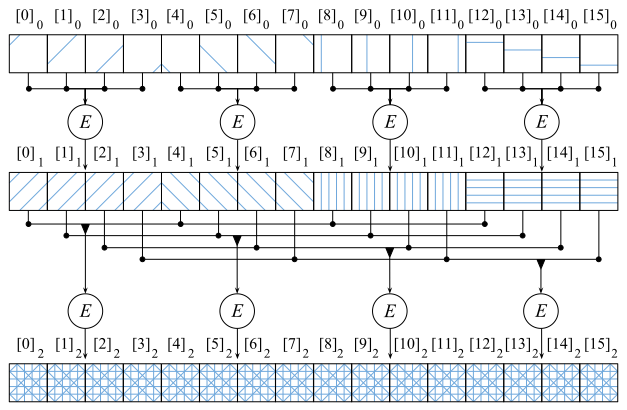
\includegraphics[width=0.7\linewidth]{images/mix_slice_example.png}
    \caption{A \textit{Mix\&Slice} example}
  \end{figure}

  % ==================================================================
  % ====================== SVILUPPO DEL PROGETTO =====================
  % ==================================================================

  \chapter{Project development}
  \thispagestyle{fancy}

  \section{Design and tools}

  The virtual file system was implemented with the Python language for the Ubuntu operating system.
  Among the libraries used in the project, the two most important are \texttt{fusepy} and \texttt{aesmix}.

  The \texttt{fusepy} \cite{fusepygithub} is a Python module that offers bindings to the C implementation
  of FUSE for Linux and macOS systems.

  The \texttt{aesmix} \cite{aesmixgithub} library provides the implementation of the \textit{Mix\&Slice} algorithm
  to encrypt and decrypt the files used during development.
  This library offers the Python \texttt{mixslice} wrapper, which permits to encrypt and decrypt a file using \textit{Mix\&Slice}.

  The Python wrapper accepts a file as input and outputs three elements:
  \begin{itemize}
    \item a directory containing the encrypted fragments produced by \textit{Mix\&Slice};
    \item a \texttt{.public} metadata file, which contains the public key;
    \item a \texttt{.private} metadata file, which contains the private key.
  \end{itemize}

  The main methods of the \texttt{aesmix} library that were used for this work belong to the \texttt{MixSlice} class
  and are the following:
  \begin{itemize}
    \item \texttt{load\_from\_file}, which loads the files needed for decryption into memory;
    \item \texttt{save\_to\_files}, which saves the various fragments and metadata files to disk;
    \item \texttt{encrypt}, to encrypt a file;
    \item \texttt{decrypt}, to decrypt a file.
  \end{itemize}

  \section{Business logic and usage}

  \subsection{Mountpoint, data folder and metadata folder}

  The virtual file system needs three directories to be mounted and used:
  \begin{enumerate}
    \item a directory indicating the mountpoint, that is, the point where the virtual file system will be mounted;
    \item a directory containing the encrypted data, possibly organised in subdirectories;
    \item a directory that contains all the metadata files (\texttt{.public}, \texttt{.private}, and \texttt{.finfo}).
  \end{enumerate}

  The directories for the encrypted files and metadata files are separate in order to allow generality
  in the use of the file system. The structure of the two must be the same to ensure uniqueness in the
  association between encrypted files and the corresponding metadata, as files with the same names can
  exist in several points of the file system.

  For example, if an encrypted file has the path \texttt{dir/image.png}, then its metadata must be
  \texttt{dir/image.png.public}, \texttt{dir/image.png.private}, and \texttt{dir/image.png.finfo}.

  Since the \texttt{aesmix} utility produces a directory containing the fragments, to distinguish between directories
  and encrypted files, the file system refers to the existence of a metadata file: for a given path,
  if the corresponding metadata file exists, then the directory is treated as if it were an encrypted file, otherwise
  its management is left to the operating system.

  \subsection{Management of encrypted files}
  \label{section-file-criptati}

  The file system must show the directories containing the encrypted fragments as files.
  To make this happen, it is necessary to change the information found in the file descriptor seen by the system.
  Since directories are files, their descriptor is retrieved in an analogous way as it is done for files (see Section \ref{filesystem-descrizione}).
  
  At the request of the descriptor by the system, the following properties are modified \cite{linuxmanstat}:
  \begin{itemize}
    \item \texttt{st\_mode}: contains permissions and file type.
          To let encrypted directories appear as files, the \texttt{S\_IFREG} flag (which identifies a file) is set,
          and the \texttt{S\_IFDIR} flag (which identifies a directory) is removed. The other permissions remain unchanged.
    \item \texttt{st\_nlink}: the number of hard links of the file.
          This is equal to $2$ for a directory, hence it is set to $1$ to make encrypted directories appear as files.
    \item \texttt{st\_size}: the size of the file in bytes.
  \end{itemize}

  In particular, in order to find the real size of a file, it is necessary to decrypt it since the operating
  system uses the \texttt{st\_size} field to know how many bytes to read from disk\footnotemark.
  In a first iteration of the project, the total size of the directory was used (i.e., the sum of the dimensions
  of the single fragments contained in it), but this caused problems when accessing the file content, especially when using a GUI.
  When the file was opened, the operating system could read fewer bytes than necessary, hence considering the file as corrupt, or
  read more bytes than necessary, leading to crashed and forced closures of applications.
  \footnotetext{This behaviour is not common throughout the whole system: it is used by the GUI but not by the command line.
  When using a terminal, even with a wrong \texttt{st\_size}, it is possible to read the content of a file
  with \texttt{cat} and to write it with a combination of \texttt{echo} and \texttt{>}.}

  However, decrypting a file every time a descriptor request is made to determine its actual size can have a significant performance impact.
  For this reason, we introduced a new metadata file type, with the extension \texttt{.finfo}, which contains
  information about the size of the file in the virtual file system.
  This size is updated at each write operation, only if it has actually changed.
  In this way, although with an initial overhead when writing to files, the file system is significantly more responsive in its normal use.
  
  What is described in this Section can only be done if it is possible to open and decrypt the file
  and if there are any metadata files associated with it.
  The directories that do not contain the encrypted fragments are therefore processed directly by the system,
  which manages them without any intervention by the virtual file system.

  \subsection{Reading, writing, and creating files}

  In order to read and write a file, it must be first opened. That is, it must be decrypted and its content transferred in memory.

  The \textit{reading} takes place in blocks on the content in memory, through an offset and a total
  number of bytes to read.
  \textit{Writing}, on the other hand, takes place via a buffer containing the data to be saved and an offset indicating
  the position of the byte to start writing from.
  It is also possible to \textit{truncate} a file, or to limit its length to a certain value.
  When opening a file, a new value must be assigned to \texttt{st\_atime}, which indicates the time instant
  of the last access to the file \cite{linuxmanstat}.

  \textit{Writing} has the particularity of not being carried out directly on mass memory, but it is done on the
  representation of the file in main memory. The file is encrypted on disk at a later time, when the file is
  flushed. For the sake of efficiency, flushing is done only if changes have been made to the file content,
  that is, if at least one write operation has been executed.
  In this way, if a file has not been modified since it was opened, no unnecessary encryptions are made,
  improving the efficiency of read-only operations.
  Writing also requires to change the value of \texttt{st\_mtime}, which indicates the instant (Unix timestamp)
  of the last modification \cite{linuxmanstat} of the file content.

  \textit{Creating} a file on disk corresponds to creating an area in memory with the necessary content,
  even empty\footnote{When creating an already existing or an already opened file, its content must be
  kept and not overwritten.}, and ``force flushing'' the file.
  Moreover, file creation enables the ability to copy and duplicate files, as copying is essentially a creation
  followed by one or more write operations.

  \subsection{Renaming and deleting files}

  \textit{Renaming} an encrypted file also renames the associated metadata files.
  If done from a graphical interface, the operation does not allow a user to rename to an already
  existing file, while from the command line the renaming is indistinguishable from moving a file.
  The implementation of a correct renaming operation therefore enables both the ability to move
  files and the ability to overwrite files in the virtual file system.

  Permanent \textit{deletion} of a file also involves deleting the metadata files. Moving a file
  to the trash bin, on the other hand, is actually a move operation, hence supported with renaming.
  If on the virtual volume created by FUSE there does not exist a directory used as a trash bin,
  this will be created. Even the files in the trash bin will be encrypted.
  
  Neither the deletion nor the renaming operations need to open and close files, therefore they are
  particularly efficient due to the absence of the encryption and decryption steps.
  Both the operations, however, need to change the information kept in memory regarding various file
  characteristics, to avoid referring to data which is no longer valid
  (see the management of \texttt{st\_size} in Section \ref{section-file-criptati} and the implementation
  of \texttt{EncFilesManager} in Section \ref{enc-files-manager}).
  It can also happen that a file is renamed while it is open.

  \subsection{Concurrency in opening a file}
  \label{aperture-multiple-file}

  A file can be opened at the same time by multiple applications. When closing any one of
  these, the file system prevents a file from being closed if it is still in use by other programs,
  in order to avoid anomalies or data corruption.

  This translates into the need to maintain a counter for each open file in memory, which is increased
  at each opening and decreased at each closure of the file.
  The file is eventually closed, releasing all the dedicated memory areas, when this counter reaches the value 0.
  It remains possible to flush the file multiple times to update its content on disk.

  The various applications take care themselves of updating the content of the file if this has
  changed on disk, or they offer the user the option to reload it.
  This happens thanks to the update of \texttt{st\_mtime} during write operations.

  \subsection{Directory management}

  To keep the exact same structure between the directory with the encrypted files and
  the directory with metadata files, the virtual file system must take care of replicating
  all directory operations (create, edit and delete) between the two locations on disk.

  This management does not present particular difficulties, except for the rename operation,
  as it is carried on directories by the operating system through the same primitive
  used for files, \texttt{rename}.
  This is different from other operations: for example, to remove a file the \texttt{unlink} method
  is used, whereas to remove a directory the \texttt{rmdir} operation is used.
  In the case of renaming, it is therefore necessary to differentiate between an encrypted file and a directory
  through the \texttt{st\_mode} property of the appropriately modified descriptor, as explained in Section \ref{section-file-criptati}.

  \subsection{Multithreading}

  The \texttt{libfuse} Linux library permits to mount virtual file systems in two ways:
  \begin{enumerate}
    \item \textit{single-thread}, where the entire file system runs on only one thread inside one process;
    \item \textit{multi-thread}, in which the various operations (writing, reading, etc.) are assigned each time to different threads.
  \end{enumerate}

  The single-thread mode is less powerful from a performance point of view, but it is simpler
  and more suitable for development, since it requires no checking of concurrency conflicts.

  The multi-thread mode instead offers better performance, as it permits to parallelize file operations
  whenever possible, such as in the case of reading a large amount of data.
  Specifically, the \texttt{libfuse} library protects the critical sections of the code from concurrent
  access through semaphores, implemented according to the POSIX standard, through the \texttt{pthread.h} library.

  \textit{FreyaFS} maintains these two paradigms, operating by default on a single thread.
  Although \texttt{libfuse} already takes care of the protection of critical sections at a low level,
  it is still necessary to protect access to shared memory areas, mainly represented by the content of
  open files and counters of applications that have opened a given file.

  The file system handles the action of writing and reading of open files differently.
  More readings can take place in parallel in order to increase performance, while writes must
  not interfere with each other and must have exclusive access to the resource.
  This behaviour is accomplished through the use of \textit{read locks} and \textit{write locks}.
  The virtual file system keeps for each open file a counter of how many threads are reading the resource:
  this is incremented every time a thread starts the read operation and decremented when it ends.
  When a thread requires write access to the file, it is put on hold if there are any readers present
  and is notified when there are no more. If instead the resource is free, exclusive access is guaranteed
  through a semaphore.

  \section{Implementation}

  The core of the project is made up of five files:

  \begin{itemize}
    \item \texttt{main.py}, which handles command line arguments and mounts the file system;
    \item \texttt{freyafs.py}, which manages the operations of the file system in general and communicates with the operating system;
    \item \texttt{encfilesmanager.py}, which implements the various input/output operations on files;
    \item \texttt{encfilesinfo.py}, which manages the \texttt{.finfo} metadata files;
    \item \texttt{filebytecontent.py}, which manages concurrent accesses to files.
  \end{itemize}

  Figure \ref{struttura-statica} shows the static structure of the code and how modules are related to each other.
  An arrow from module A to module B indicates that B uses module A.
  In the ``external'' modules we have the \texttt{aesmix} library, which implements \textit{Mix\&Slice}, and
  \texttt{fusepy}, which provides the implementation of FUSE for the Python language.
  The ``internal'' modules are those managing the encrypted files and realise the logic of the virtual file system.
  Finally, \texttt{main} only handles the interface with the user from the command line and invokes
  \texttt{fusepy} to mount the file system.

  \begin{figure}
    \centering
    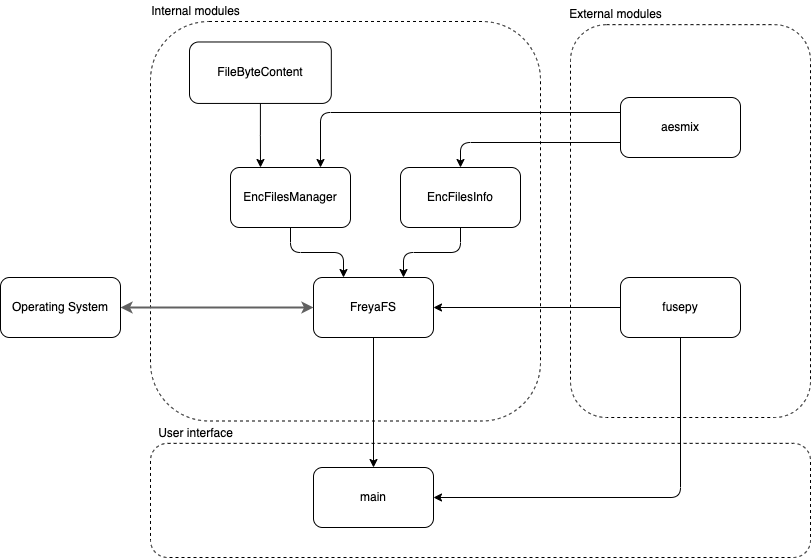
\includegraphics[width=0.8\linewidth]{images/code-diagram-en.png}
    \caption{Code structure}
    \label{struttura-statica}
  \end{figure}

  \subsection{User interaction}

  User interaction is managed by the \texttt{main.py} module, which is responsible to process
  the parameters passed on the command line and to mount the file system.
  The available parameters are shown in Table \ref{table-main}.

  \begin{table}[h!]
    \centering
    \begin{tabular}{|p{4.5cm}|p{9.5cm}|} 
      \hline
      Parameter & Description \\ [0.5ex] 
      \hline\hline
      \texttt{MOUNT} & The mountpoint, the path where the file system will be mounted \\ 
      \hline
      \texttt{-{}-data DATA} & The path to the directory containing the encrypted files \\
      \hline
      \texttt{-{}-metadata METADATA} & The path to the directory containing the metadata files \\
      \hline
      \texttt{-{}-multithread} & Flag indicating whether to mount the file system in multi-thread mode (default to \texttt{False}) \\
      \hline
    \end{tabular}
    \caption{\texttt{main.py} parameters}
    \label{table-main}
  \end{table}
  
  
  \subsection{FreyaFS}

  The \texttt{freyafs} module implements FUSE's methods for managing the virtual file system.
  In particular, the most important part of the module is the \texttt{FreyaFS} class, that extends
  the FUSE \texttt{Operations} class and overrides some methods.
  A lot of the methods of the class simply call the operating system, as they do not require encryption support
  (such as the test to access a file).
  Other methods are redefined to support the file encryption and decryption, performed by the
  \texttt{encfilesmanager} module.
  
  What follows is an extract of the \texttt{getattr} method, used to obtain information about
  files and folders. The code visible here focuses on the modification of the descriptor's information
  about the folders containing the encrypted fragments.

  \begin{lstlisting}[language=Python]
  if full_path not in self.enc_info:
    public_metadata, _, finfo = self._metadata_names(path)
    self.enc_info[full_path] = EncFilesInfo(full_path, public_metadata, finfo)

  return {
      'st_mode': stat.S_IFREG | (st.st_mode & ~stat.S_IFDIR),
      'st_nlink': 1,
      'st_atime': st.st_atime,
      'st_ctime': st.st_ctime,
      'st_gid': st.st_gid,
      'st_mtime': st.st_mtime,
      'st_size': self.enc_info[full_path].size,
      'st_uid': st.st_uid
  }
  \end{lstlisting}

  The main duties of this code snippet are two: to calculate the size of the encrypted file, and to
  change the flags so that the folder containing the fragments appears as a single file.

  The size calculation is done through instantiating the \texttt{EncFilesInfo} class and
  only if not already done before (in order to improve performance, rows from 1 to 3).
  The \texttt{self.enc\_info} property is a dictionary containing the various \texttt{EncFilesInfo} instances,
  one for every encrypted file found in the system.
  
  The flag change is done so that the same access rights are kept, as visible in row 6,
  represented by \texttt{st.st\_mode}, which is the set of permissions of the original folder.
  The \texttt{stat.S\_IFREG} is set to 1 through a bit-by-bit \texttt{OR} operation, while to remove
  the \texttt{stat.S\_IFDIR} it is necessary to do a bit-by-bit \texttt{AND} with the bit-by-bit negation
  of \texttt{stat.S\_IFDIR}.

  The following snippet shows an extract of the \texttt{unlink} method, used to remove files.

  \clearpage
  \begin{lstlisting}[language=Python]
  full_path = self._full_path(path)
  public_metadata, private_metadata, finfo = self._metadata_names(path)

  os.unlink(public_metadata)
  os.unlink(private_metadata)
  if os.path.isfile(finfo):
      os.unlink(finfo)

  if full_path in self.enc_info:
      del self.enc_info[full_path]

  shutil.rmtree(full_path)
  \end{lstlisting}

  In this code there are only calls to the operating system primitives, without opening nor closing any file.
  The metadata files are also deleted, and the associated memory areas are freed (row 10).
  It is also necessary to check whether the \texttt{.finfo} file exists (row 6) because, unlike \texttt{.public}
  and \texttt{.private} files, it may not exists as it is created on the first \texttt{getattr} call.

  The \texttt{rename} methods manages the renaming of a file, which is more complex, since
  it is the same operation for both files and folders.
  Moreover, due to the encrypted files being actually folders, if one wants to rename a file
  to another already existing file\footnote{This is prohibited when using a GUI, but allowed through the command line \texttt{mv} command.}
  it is necessary to delete the latter (rows 6-7), in order to prevent the system from recognising it as a folder
  and moving the former ``into'' the latter.
  Lastly, the in-memory paths relative to the file and its metadata files are renamed (rows 19-25).

  When dealing with ``regular'' folders, i.e., those not containing encrypted fragments,
  the rename is left to the operating system and replicated both in the encrypted files path
  and in the metadata files path (the \texttt{else} branch).

  \clearpage
  \begin{lstlisting}[language=Python]
  full_old_path = self._full_path(old)
  full_new_path = self._full_path(new)

  if self._is_file(old):
      if self._is_file(new):
          self.unlink(new)

      old_public_metadata, old_private_metadata, old_finfo = self._metadata_names(old)
      new_public_metadata, new_private_metadata, new_finfo = self._metadata_names(new)

      os.rename(old_public_metadata, new_public_metadata)
      os.rename(old_private_metadata, new_private_metadata)
      if os.path.isfile(old_finfo):
          os.rename(old_finfo, new_finfo)

      os.rename(full_old_path, full_new_path)

      if full_old_path in self.enc_files:
          self.enc_files.rename(full_old_path, full_new_path)
      
      if full_old_path in self.enc_info:
          self.enc_info[full_old_path].rename(full_new_path, new_public_metadata, new_finfo)
          self.enc_info[full_new_path] = self.enc_info[full_old_path]
          del self.enc_info[full_old_path]
  else:
      old_metadata_path = self._metadata_full_path(old)
      new_metadata_path = self._metadata_full_path(new)            
      os.rename(old_metadata_path, new_metadata_path)
      os.rename(full_old_path, full_new_path)
  \end{lstlisting}

  All methods that act on file input and output all act as a proxy to the \texttt{EncFilesManager}
  methods and, if necessary, update the relative size managed by \texttt{EncFilesInfo}.
  As an example, the following snippet shows the \texttt{write} method.

  \clearpage
  \begin{lstlisting}[language=Python]
  def write(self, path, buf, offset, fh):
      full_path = self._full_path(path)
      if full_path in self.enc_files:
          bytes_written = self.enc_files.write_bytes(full_path, buf, offset)
          self._update_enc_file_size(full_path)
          return bytes_written

      os.lseek(fh, offset, os.SEEK_SET)
      return os.write(fh, buf)
  \end{lstlisting}
  
  In this two extracts, \texttt{self.enc\_files} is an instance of the \texttt{EncFilesManager} class,
  which contains all the contents of the currently opened files.

  The \texttt{open}, \texttt{create}, \texttt{truncate}, \texttt{read}, \texttt{flush}, and \texttt{release} methods
  all have a similar structure. If an open file is not among those encrypted, then the file is managed by the operating
  system as it normally would.

  In conclusion, Table \ref{table-freyafs} summarises the methods used by \textit{FreyaFS} that were changed
  with respect to the basic case, where each method simply invokes the corresponding primitives of the operating system.

  \begin{table}[h!]
    \centering
    \begin{tabular}{|p{3cm}|p{11cm}|} 
      \hline
      Method & Goal \\ [0.5ex] 
      \hline\hline
      \texttt{getattr} & Retrieve the properties of an encrypted file or directory \\ 
      \hline
      \texttt{readdir} & Retrieve the content of a given directory, including the \texttt{.} and \texttt{..} entries, and ignoring metadata files \\
      \hline
      \texttt{mkdir} & Create a directory, both in the encrypted data path and in the metadata path \\
      \hline
      \texttt{rmdir} & Remove a directory, both in the encrypted data path and in the metadata path \\
      \hline
      \texttt{unlink} & Remove an encrypted file, also deleting the corresponding metadata files \\
      \hline
      \texttt{rename} & Rename an encrypted file (and corresponding metadata files) or a directory \\
      \hline
      \texttt{utimens} & Update the instants of the last update and the last editing for encrypted files and directories \\
      \hline
      \texttt{open} & Open an encrypted file \\
      \hline
      \texttt{create} & Create an encrypted file \\
      \hline
      \texttt{read} & Read a certain number of bytes from an encrypted file \\
      \hline
      \texttt{write} & Write a certain number of bytes from an encrypted file \\
      \hline
      \texttt{truncate} & Truncate the content of an open encrypted file at a given length \\
      \hline
      \texttt{flush} & Force writes made to an encrypted file from memory to disk \\
      \hline
      \texttt{release} & Release an open encrypted file \\
      \hline
    \end{tabular}
    \caption{\textit{FreyaFS}'s methods}
    \label{table-freyafs}
  \end{table}

  \subsection{EncFilesManager}
  \label{enc-files-manager}

  This module defines the class with the same name managing the input and output on encrypted files.
  Specifically, the class is instantiated only once and contains information on all files
  (encrypted with \textit{Mix\&Slice}) currently open, identifiable by their path in the real file system.
  It makes use of a counter for each open file that indicates how many applications are currently using it:
  this way, the class avoids to accidentally close a file if only some of these applications have released it
  while others have it still open.

  The offered methods are the following:
  \begin{itemize}
    \item \texttt{open}: opens a file, decrypting its content and keeping it in memory;
    \item \texttt{create}: creates an empty file, i.e., it reserves empty space in memory for the content of the file
          (only if not already open) and flushes it;
    \item \texttt{read\_bytes}: reads a certain number of bytes from an open file;
    \item \texttt{write\_bytes}: overwrites part of the content of an open file with data contained in a buffer;
    \item \texttt{truncate\_bytes}: truncates the content of an open file to a certain length;
    \item \texttt{flush}: writes the content of an open file to disk, encrypting it;
    \item \texttt{release}: releases the memory areas dedicated to a file, closing it;
    \item \texttt{cur\_size}: gets the current length of the content of an open file;
    \item \texttt{rename}: renames the various paths referring to an open file.
  \end{itemize}

  It is essential to have a \texttt{rename} method, because a file can be renamed even if open:
  in this case, to avoid referencing files that no longer exist and cause the file system to behave incorrectly,
  it is necessary to update all the paths related to the file in question.
  
  The \texttt{EncFilesManager} class also tracks the change status of a file using Boolean flags.
  That way, if a \texttt{flush} is requested but there are no changes to the file,
  the encryption operation can be skipped, improving performance and avoiding wasted time.

  Finally, the class also handles mutual exclusion for the multi-thread mode of the virtual file system,
  via a \texttt{Lock} semaphore of the Python \texttt{threading} module (see Section \ref{section-lib-threading}).
  This semaphore guarantees exclusive access to structures containing the content of open files and open file counters.

  The following code snippet shows the implementation of the \texttt{open} method:
  \begin{lstlisting}[language=Python]
  def open(self, path, public_metafile_path, private_metafile_path, mtime):
    with LOCK:
        if path in self.open_files:
            self.open_counters[path] += 1
            return

        self.public_metafiles[path] = public_metafile_path
        self.private_metafiles[path] = private_metafile_path

        self.open_files[path] = FileByteContent(self._decrypt(path))
        self.open_counters[path] = 1
    
    self.touched_files[path] = False
    self.atimes[path] = int(time())
    self.mtimes[path] = mtime
  \end{lstlisting}

  The method also takes care of updating the ``last accessed'' timestamp for a file
  via \texttt{self.atimes}, and the ``last changed'' timestamp via \texttt{self.mtimes}.
  Between the two, only the latter is updated when writing the file, while both of them
  are always updated when flushing, even without any change to the file content.

  \subsection{EncFilesInfo}

  The \texttt{encfilesinfo} module defines the \texttt{EncFilesInfo} class,
  which is responsible of the management of information about the encrypted files that
  is not contained in the \texttt{.private} and \texttt{.public} metadata files.
  Its main job is to interface \texttt{freyafs} with \texttt{.finfo} files,
  which contain information serialised in the JSON format.
  Unlike the \texttt{EncFilesManager} class, the \texttt{EncFilesInfo} class is not aware of
  all the files managed by the virtual file system, but it only manages the information of a single file specified at initialisation.

  Specifically, the module supports the management of the length in bytes of the content of the encrypted file,
  which can be obtained and set using the property \texttt{size}.
  
  When the class is instantiated, the size of the desired encrypted file is calculated and
  is stored in the \texttt{size} property and also in the \texttt{.finfo} file (which, if not present, is created).
  When this property is updated, the value contained in the metadata file is also updated,
  but only if the value is different from the previous one.
  This avoids opening a file, parsing the JSON contained in it, updating the property
  and then serialising the JSON produced, in case these operations are not strictly necessary.
  
  \clearpage
  \begin{lstlisting}[language=Python]
  @property
  def size(self):
      if self._size is None:
          self._size = size_decrypt(self._path, self._public_metadata)
          self._update_finfo()
      return self._size

  @size.setter
  def size(self, value):
      if self._size == value:
          return
      self._size = value
      self._update_finfo()
  \end{lstlisting}

  The class also provides a \texttt{rename} method, used to rename the path to the file containing this information.

  \subsection{FileByteContent}
  \label{section-filebytecontent}

  This module deals with reading and writing the content of a file opened in a mutually exclusive way.
  To ensure this, the \texttt{FileByteContent} class has the following properties:
  \begin{itemize}
    \item \texttt{\_text}, which represents the content of the file as a string of bytes;
    \item \texttt{\_readers}, which indicates the number of current readers in a given moment;
    \item \texttt{\_cond}, of type \texttt{threading.Condition}, which is used as a semaphore.    
  \end{itemize}

  The \texttt{FileByteContent} class uses a semaphore for each open file
  In this way, parallel reads and writes to different files are possible, but not on the same file.

  As an example, the following are some of the methods of the class.
  
  \begin{lstlisting}[language=Python]
  def read_bytes(self, offset, length):
      self._r_acquire()
      text = self._text[offset:offset + length]
      self._r_release()
      return text

  def write_bytes(self, buf, offset):
      self._w_acquire()
      bytes_written = len(buf)
      new_text = self._text[:offset] + buf + self._text[offset+bytes_written:]
      self._text = new_text
      self._w_release()
      return bytes_written

  def truncate(self, length):
      self._w_acquire()
      self._text = self._text[:length]
      self._w_release()
  \end{lstlisting}

  In this snippet, methods \texttt{\_r\_acquire()} and \texttt{\_r\_release()} permit respectively
  to acquire and release the read lock, which can be shared between multiple threads,
  while methods \texttt{\_w\_acquire()} and \texttt{\_w\_release()} are the equivalent for the write lock,
  which guarantees exclusive access to the file content.
  
  The acquisition of a lock for reading increases the \texttt{\_readers} variable, which is decremented at every release.
  When value $0$ is reached, any thread waiting for a write lock is notified.
  
  When asking for a write lock on a file, the thread waits as long as there are readers, i.e.,
  if \texttt{\_readers} is positive. When all the readers have released the resource,
  the lock is acquired and then released at the end of the write operation.

  The methods for the acquisition and release of read and write locks are as follows.
  For more details on the \texttt{\_cond} property, see Section \ref{section-lib-threading}.

  \clearpage
  \begin{lstlisting}[language=Python]
  def _r_acquire(self):
      self._cond.acquire()
      try:
          self._readers += 1
      finally:
          self._cond.release()

  def _r_release(self):
      self._cond.acquire()
      try:
          self._readers -= 1
          if self._readers == 0:
              self._cond.notify_all()
      finally:
          self._cond.release()

  def _w_acquire(self):
      self._cond.acquire()
      while self._readers > 0:
          self._cond.wait()

  def _w_release(self):
      self._cond.release()
  \end{lstlisting}

  \subsection{The \texttt{threading} library}
  \label{section-lib-threading}

  The \texttt{threading} library \cite{pythreading} is a built-in Python library that
  supports the management of high-level threads and provides tools for creating and using semaphores.
  
  The classes used for \textit{read locks} and \textit{write locks} in the \texttt{FileByteContent} class
  (Section \ref{section-filebytecontent}) are:
  \begin{itemize}
    \item \texttt{threading.Lock}, which offers the implementation of the concept of mutex, a mutually exclusive semaphore;
    \item \texttt{threading.Condition}, which represents a condition associated with a particular \texttt{Lock} instance.
  \end{itemize}

  In the code of the \texttt{FileByteContent} class there is the \texttt{\_cond} property of type \texttt{Condition},
  which provides the following methods:
  \begin{itemize}
    \item \texttt{acquire}: acquires the underlying lock;
    \item \texttt{release}: releases the underlying lock;
    \item \texttt{wait}: suspends the calling thread and releases the underlying lock, which must have previously been acquired by the thread;
    \item \texttt{notify\_all}: wakes up all queued threads, which leave the wait queue only when they gain control over the lock.
  \end{itemize}
  
  The semaphores provided by \texttt{Lock} are objects that can be in a state ``locked'' or ``free''.
  When the lock is in the free state, it can be acquired through the \texttt{acquire} method, which puts it in the locked state.
  Instead, if \texttt{acquire} is invoked while the semaphore is locked, the calling
  thread pauses until a \texttt{release} call frees the mutex.

  Objects instantiated by \texttt{Condition} are more flexible than simple mutexes,
  but they are always associated with a semaphore.
  Through these objects it is possible to suspend a thread with the \texttt{wait} method, placing it in a wait queue
  and causing the underlying lock to be released, and awaken it with \texttt{notify} or \texttt{notify\_all}.
  Upon exiting the queue, the thread acquires the lock again and then continues in its execution.
  In this way, it is possible to avoid \textit{busy waits}, that is, situations in which the thread continuously
  checks the state of the semaphore, occupying computational resources that could be used by other unblocked threads.
  
  Finally, both classes support the \textit{context management protocol}, that is,
  the use of the Python \texttt{with} construct. When the process or thread enters a block delimited
  by \texttt{with}, the \texttt{acquire} method of the lock or condition is called, while at the exit the \texttt{release} method is invoked.
  This construct is visible in the implementation of the \texttt{EncFilesManager} class in Section \ref{enc-files-manager}.

  % ==================================================================
  % ====================== TESTING ED ANALISI ========================
  % ==================================================================

  \chapter{Testing and analysis}
  \thispagestyle{fancy}

  \section{System}

  The virtual file system was developed and tested on the following system:

  \begin{itemize}
    \item Ubuntu 20.04 LTS Focal Fossa as the operating system;
    \item a Intel Core i5-7200U quad-core 2.5 GHz CPU;
    \item 8 GB RAM;
    \item 120 GB solid state drive.
  \end{itemize}

  \section{Multiple opening of the same file}

  The opening of the same file with multiple applications has been tested on the following file formats:
  \begin{enumerate}
    \item a \texttt{.txt} text file, with \textit{gedit} and \textit{Visual Studio Code};
    \item a \texttt{.md} text file, with \textit{gedit} and \textit{Typora};
    \item a \texttt{.jpg} binary file, with \textit{Image Viewer} and \textit{Firefox};
    \item a \texttt{.pdf} binary file, with \textit{Document Viewer} and \textit{Xournal}.
  \end{enumerate}

  For \texttt{.txt} files, both the applications open
  the file and immediately close it again after reading the entire content.
  Only when the save operation is invoked, the file is opened again to make the necessary updates.
  This reduces the possibility of running into concurrency problems that may arise
  when two applications keep the same file open at the same time.
  The same exact situation occurs with \texttt{.md} files and \texttt{.jpg} files.
  Applications react differently to changes to the content on disk of an opened file:
  for example, \textit{gedit} always proposes to the user to reload the entire file,
  while \textit{Typora} and \textit{Visual Studio Code} transparently update the file and notify
  the user only if there are pending changes created by the user.
  
  The applications used to test \texttt{.pdf} files behave differently:
  both \textit{Document Viewer} and \textit{Xournal} keep the file open and only release it when it is closed.
  Specifically, \textit{Xournal} reads the content partially as the user scrolls through the document.
  For this reason, it is necessary to use the counters for open files discussed earlier in Section \ref{aperture-multiple-file},
  to avoid anomalies and concurrency problems.

  In Section \ref{enc-files-manager} it was noted that a file could be renamed while opened:
  this behaviour is visible when saving a file with \textit{gedit}: the application creates a temporary
  hidden file, opens it, updates its content, and finally renames it into the original file so to overwrite it.

  \section{Performance}

  \subsection{Measuring methods}

  The execution times were measured to estimate the performance of some common operations, computed on the basis of 150 tests.

  To automate the measurements, we used dedicated Python scripts.
  The files needed for testing are text files created randomly using
  the command \texttt{base64 /dev/urandom | command head -c BYTES > FILENAME.txt}.

  \clearpage
  \begin{lstlisting}[language=Python]
  times = []
  for i in range(150):
      start = msnow()
      with open(filename) as f:
          end = msnow()
          times.append(start - end)

  times = []
  for i in range(150):
      with open(filename) as f:
          start = msnow()
          data = f.read()
          end = msnow()
          times.append(start - end)


  times = []
  f = open(filename, 'r+')
  content = f.read()
  for i in range(150):
      f.seek(0)
      start = msnow()
      f.write(content)
      end = msnow()
      f.truncate()
      times.append(start - end)
  f.close()
  \end{lstlisting}
  
  In the Python snippet, \texttt{msnow} is a function that returns the Unix timestamp in milliseconds,
  while \texttt{times} is a list used to calculate expected values and standard deviations.

  Write times are measured by overwriting the entire file: for one file of size $D$ bytes, the bytes written to disk are exactly $D$.

  \subsection{Execution times}

  Tables \ref{table:t-open}, \ref{table:t-read}, and \ref{table:t-write} show the mean $\mu$ and standard deviation $\sigma$
  of the execution times of some common operations, obtained through the scripts described
  in the previous section, comparing \textit{FreyaFS} in single-thread mode with the direct use of the operating system.

  \begin{table}[h!]
    \centering
    \begin{tabular}{|r||r|r||r|r|} 
      \hline
      File size & $\mu_\text{FreyaFS}$ [ms] & $\sigma_\text{FreyaFS}$ [ms] & $\mu_\text{OS}$ [ms] & $\sigma_\text{OS}$ [ms] \\ [0.5ex]
      \hline\hline
      4 KB & 13.57 & 0.69  & 0.01 & 0.11 \\
      \hline
       1 MB & 13.60 & 0.52 & 0.01 & 0.11 \\
      \hline
      10 MB & 71.05 & 2.04 & 0.01 & 0.11 \\
      \hline
    \end{tabular}
    \caption{Opening times}
    \label{table:t-open}
  \end{table}

  \begin{table}[h!]
    \centering
    \begin{tabular}{|r||r|r||r|r|} 
      \hline
      File size & $\mu_\text{FreyaFS}$ [ms] & $\sigma_\text{FreyaFS}$ [ms] & $\mu_\text{OS}$ [ms] & $\sigma_\text{OS}$ [ms] \\ [0.5ex]
      \hline\hline
      4 KB & 0.11 & 0.35   & 0.01 & 0.11 \\
      \hline
      1 MB & 1.22 & 0.54   & 0.38 & 0.79 \\
      \hline
      10 MB & 8.85 & 0.84  & 5.21 & 2.38 \\
      \hline
    \end{tabular}
    \caption{Reading times}
    \label{table:t-read}
  \end{table}

  \begin{table}[h!]
    \centering
    \begin{tabular}{|r||r|r||r|r|} 
      \hline
      File size & $\mu_\text{FreyaFS}$ [ms] & $\sigma_\text{FreyaFS}$ [ms] & $\mu_\text{OS}$ [ms] & $\sigma_\text{OS}$ [ms] \\ [0.5ex]
      \hline\hline
      4 KB & 0.14 & 0.30    & 0.01 & 0.08 \\
      \hline
      1 MB & 69.08 & 8.97   & 0.26 & 0.44 \\
      \hline
      10 MB & 12203 & 95    & 4.54 & 0.62 \\
      \hline
    \end{tabular}
    \caption{Writing times}
    \label{table:t-write}
  \end{table}

  Looking at the times of \textit{FreyaFS}, reading turns out to be quite faster than writing.
  This behaviour is due to how the virtual file system works: a file is decrypted upon opening and
  its content is then kept in memory until each file is closed. The reading then takes place on data
  present in RAM and not from disk, thus offering almost immediate access.

  In the measurements of the operating system, however, the opening appears to be with good approximation
  always the same and much less than the opening with \textit{FreyaFS}.
  This happens because with FreyaFS opening also involves reading each of the fragments and
  decrypting them, operations that slow down execution.
  A similar note can be done about the write operation: the encryption of all of the new content
  introduces more delays.

  % ==================================================================
  % ====================== CONCLUSIONI ===============================
  % ==================================================================

  \chapter{Conclusions}
  \thispagestyle{fancy}

  \textit{FreyaFS} is meant to create a virtual file system for the GNU/Linux
  operating system that supports encryption through \textit{Mix\&Slice}.
  This project has been divided into two phases that were always side by side with
  development and code production: an analysis of the file system, and the
  management of concurrency in a Linux kernel.

  Firstly, it was necessary to study how the FUSE library and how a real file system work,
  in order to allow communication between the two and make as transparent as possible
  the interaction with the user. Specifically, the analysis of the operating system's file management
  was a substantial part of the project at multiple levels of abstractions:
  how to handle file descriptors at a low-level, and how to interface with a graphical shell
  at a high-level.

  Secondly, semaphores were crucial in order to allow concurrent accesses to the same file
  by different applications and to sync accesses to resources that are shared between threads.
  The read/write lock implementation proved useful to protect resources from
  concurrency problems.

  The virtual file system developed in this thesis work realises correctly
  the fundamental functions of managing files and folders, i.e., creating,
  deleting, moving, and modifying them.
  The main advantage that \textit{FreyaFS} brings is its \textit{encrypted} nature,
  since it manages data while guaranteeing privacy thanks to innovative and secure
  encryption methods such as \textit{Mix\&Slice}.

  % ==================================================================
  % ====================== BIBLIOGRAFIA ==============================
  % ==================================================================

  \nocite{*}
  \printbibliography[heading=bibintoc]
  \thispagestyle{fancy}
\end{document}
